\graphicspath{{general_design/fig/}}

\chapter{Design}
\label{chap:general_design}

\begin{figure}[!h]
    \centering
    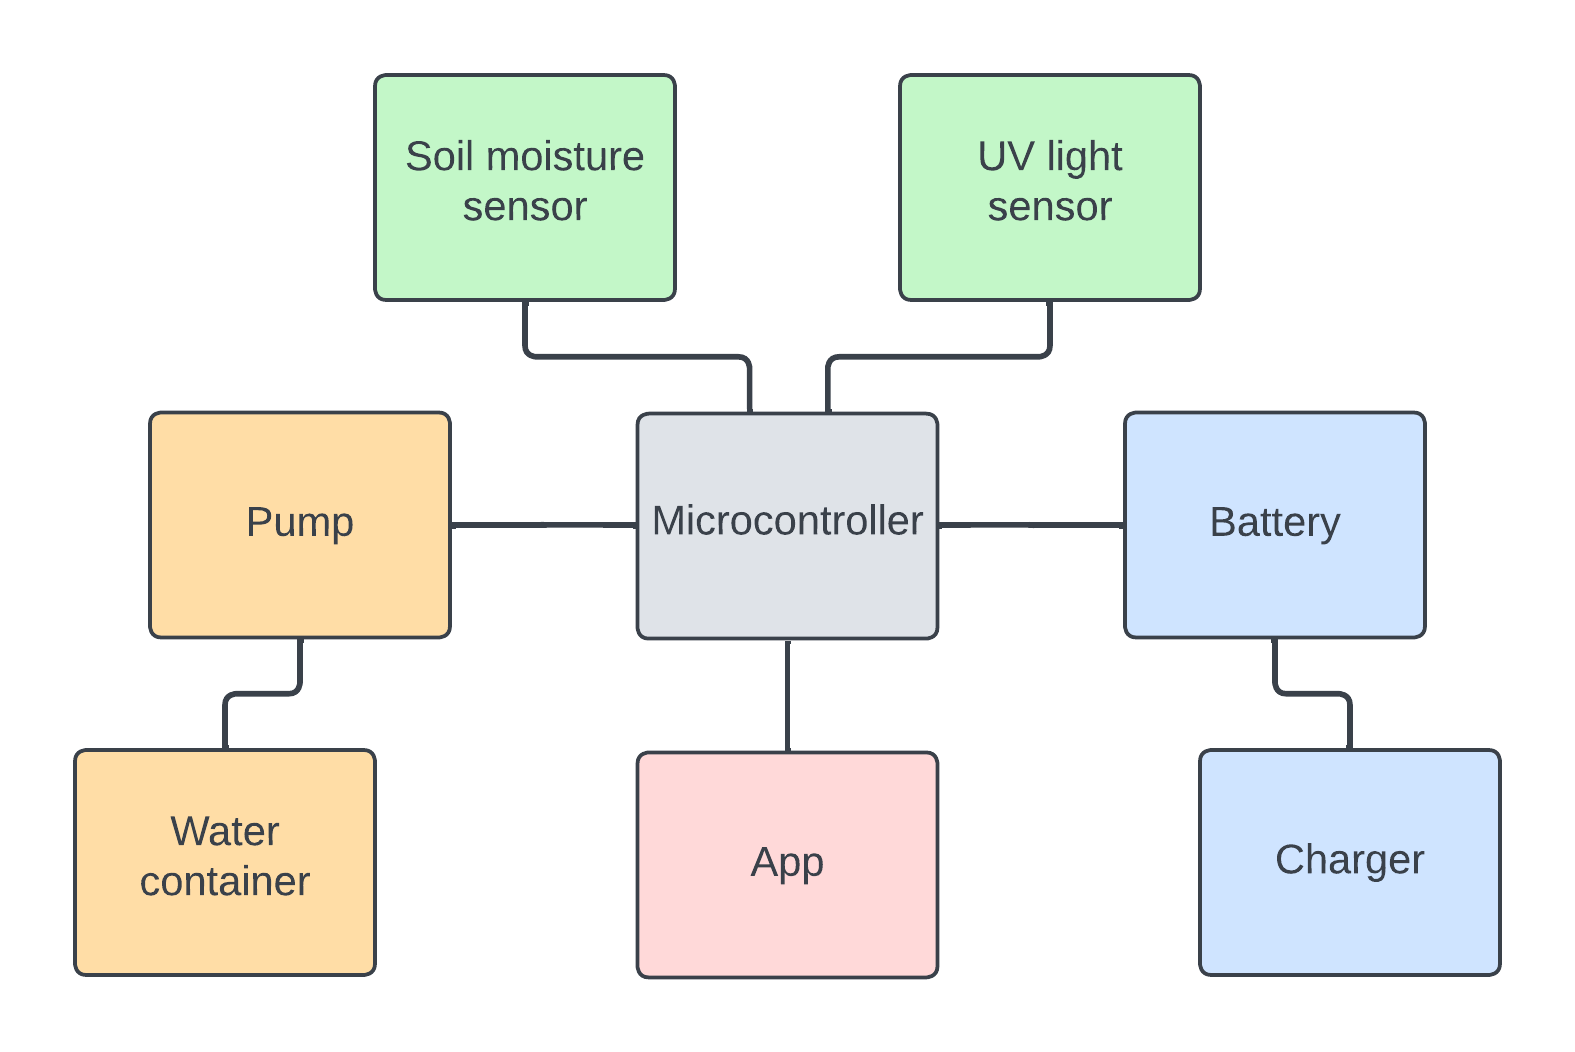
\includegraphics{design_diagram.png}
    \caption{System design overview}
    \label{fig:design_overview}
\end{figure}

This chapter describes the general requirements and design of the system. This includes the design and interactions of sub-systems as well as the selection of major components. Detailed design decisions and processes are described in chapter \ref{chap:detail_design}.

%%%%%%%%%%%%%%%%%%%%%%%%%%%%%%%%%%%%%%%%
\section{Requirements}
The project is intended for indoor use and must therefore be designed to be as small and compact as possible. \\

To function during power outages, the system will need to include a battery that can be recharged from a standard power outlet. \\

The system must be able to reliably and accurately monitor soil moisture levels and exposure to sunlight. This data must be accessible to the user and presented in a way that is easy to understand. \\

The system must be able to reliably maintain soil moisture levels by providing water automatically. The user must be able to adjust the desired soil moisture level.

%%%%%%%%%%%%%%%%%%%%%%%%%%%%%%%%%%%%%%%%
\subsection{UV light exposure and soil moisture level
measurement and logging}
The system must be able to log the average soil moisture and \ac{UV} light exposure levels every minute. This data must be uploaded to be viewed on the app every 30 minutes.

%%%%%%%%%%%%%%%%%%%%%%%%%%%%%%%%%%%%%%%%
\section{System design and component selection}

Data from a soil moisture and \ac{UV} light sensor will be monitored using a microcontroller. When soil moisture levels fall below a set value, a pump will turn on to water the plant until the soil reaches the target moisture level. The soil moisture, \ac{UV} light exposure and watering times will be logged by the microcontroller and sent to a server. The user can use the app to view the data and set the moisture level target. The system will be powered by a battery that charges when power is available.

\begin{table}[!h]
    \centering
    \begin{tabular}{|c|c|c|c|}
        \hline
        Component & Selected & Cost & Product page \\
        \hline
        Microcontroller &  ESP32 C6 Dev Board & R 285.20 & \href{https://www.robotics.org.za/ESP32-C6-DEV}{link} \\
        UV light sensor & Wave UV Sensor Module - GUVA-S12D & R 112.70 & \href{https://www.robotics.org.za/W9537}{link} \\
        Soil moisture sensor & Capacitive Soil Moisture Sensor V1.2 & R 55.20 & \href{https://www.robotics.org.za/CAP-SW-12}{link} \\
        Pump & Digital Peristaltic Pump & R 879.95 & \href{https://www.diyelectronics.co.za/store/dfrobot/2119-digital-peristaltic-pump.html?search_query=PERISTALTIC+PUMP&results=4}{link} \\
        Battery & Li-polymer Battery HAT - 5V output & R 399.95 & \href{https://www.diyelectronics.co.za/store/hats/2726-lipo-battery-hat-5v-output.html?search_query=Li-polymer+Battery+HAT&results=14}{link}\\
        \hline
        Total & & R 1 733.00 & \\
        \hline
    \end{tabular}
    \caption{Selected components}
    \label{tab:components_selected}
\end{table}

%%%%%%%%%%%%%%%%%%%%%%%%%%%%%%%%%%%%%%%%
\subsection{Microcontroller}
Data will be sent from the microcontroller to the app using a web server. This requires the microcontroller to be connected to a WiFi network. A Bluetooth connection will be used to initially connect the microcontroller to a WiFi network.

The selection of microcontrollers with a reasonable shipping time and cost are limited. The ESP32 C6 Dev Board was selected as it has both Bluetooth and WiFi capabilities.


%%%%%%%%%%%%%%%%%%%%%%%%%%%%%%%%%%%%%%%%
\subsection{\Ac{UV} light and soil moisture sensing}
A capacitive soil moisture sensor will be used as they do not rust like resistive sensors do when exposed to moisture for extended time periods. This will allow the sensor to be left in the soil permanently. Both the soil moisture sensor and \ac{UV} light sensor can be connected to a microcontroller without any additional circuits and output a measurement equivalent analog voltage. 

%%%%%%%%%%%%%%%%%%%%%%%%%%%%%%%%%%%%%%%%
\subsection{Automatic watering}
The pump will be powered by the battery. A driver circuit allows the pump to be controlled using the microcontroller. A peristaltic pump will be used to prevent siphoning. \\

Siphoning could also be prevented by using valves along with a small centrifugal pump, potentially resulting in a lower cost. A peristaltic pump will, however lead to a more compact system as it does not need to be submerged and can be contained within the same casing as the rest of the system. \\

The digital peristaltic pump was selected as it includes a drive circuit that takes a \ac{PWM} voltage as input and requires only 5W at 5V to function.

%%%%%%%%%%%%%%%%%%%%%%%%%%%%%%%%%%%%%%%%
\subsection{App}
The app will allow the user to view the \ac{UV} light exposure, soil moisture levels and watering over times. The app will also allow the user to connect the microcontroller to WiFi initially and change the target soil moisture level. Figure \ref{fig:app_flow_rough} shows the initial design of the app. 

\begin{figure}[!h]
    \centering
    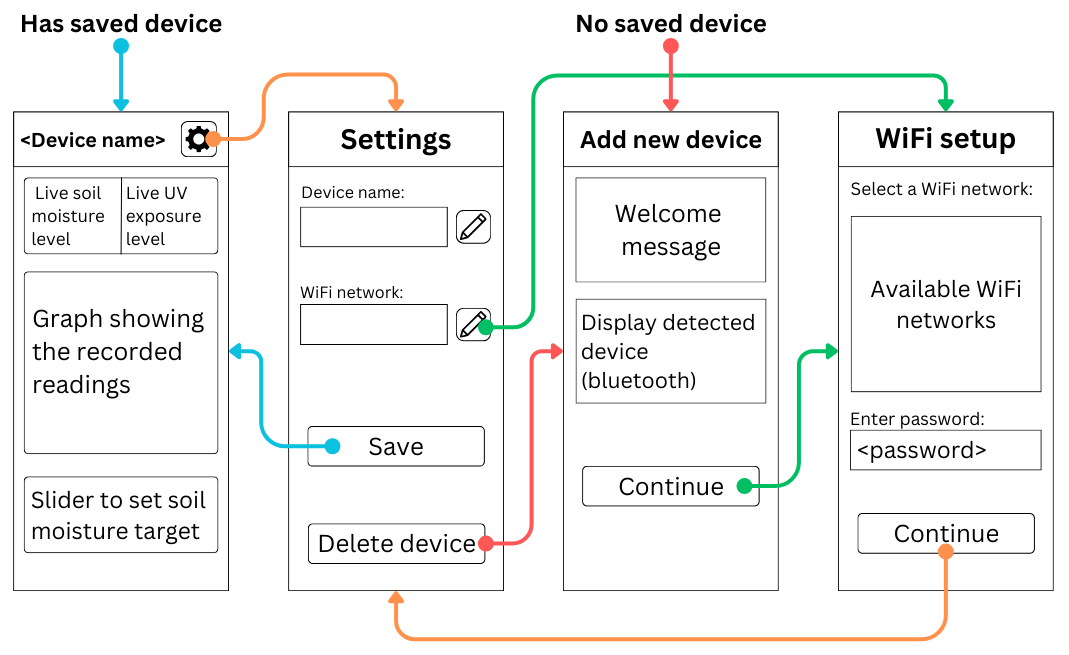
\includegraphics[width= \textwidth]{Report/general_design/fig/app_flow_rough.png}
    \caption{Initial app design}
    \label{fig:app_flow_rough}
\end{figure}



%%%%%%%%%%%%%%%%%%%%%%%%%%%%%%%%%%%%%%%%
\subsection{Battery and charging}
The battery will need to be able to power the system for at least two hours at a time to ensure the system functions during loadshedding. The battery needs to be charged whenever power is available. 
\\

Two commonly available battery types were considered: Lithium-ion and lead-acid. The following factors were compared in table \ref{tab:battery_comp}: 

\begin{itemize}
    \item \textbf{Cost:} The initial cost of the battery
    \item \textbf{Depth of discharge:} Maximum percentage of a fully charged battery that can be used before recharging
    \item \textbf{Cycle life:} The amount of charge/discharge cycles the battery can undergo without performance being affected
    \item \textbf{Power delivery:} The amount of power delivered in a charge cycle
    \item \textbf{Size:} Physical size of the battery
\end{itemize}

\begin{table}[!h]
    \centering
    \begin{tabular}{|c||c|c|}
        \hline
         &  Lead-acid & Lithium-ion \\
        \hline
        Cost & Costs less & Costs more \\
        Depth of discharge \cite{battery_10_diff} & 50\% & 80\% \\
        Cycle life \cite{battery_10_diff} & 300 - 500 cycles & 5000 cycles \\
        Power delivery \cite{battery_guide} & Starts strong but dissipates & Constant \\
        Size \cite{battery_10_diff} & Larger & Smaller \\
        \hline
    \end{tabular}
    \caption{Lithium-ion and lead-acid battery comparison}
    \label{tab:battery_comp}
\end{table}

The Li-Polymer battery HAT was chosen as it provides a 5V, 1.8A output \cite{battery_faq} and manages the charging of the included battery. The battery has a 3000mAh capacity and will be able to provide power to the system throughout loadshedding provided that the pump is not running constantly.

%%%%%%%%%%%%%%%%%%%%%%%%%%%%%%%%%%%%%%%%
\subsection{PCB}
To keep the final system as compact as possible, a PCB will be designed for the circuits.

%%%%%%%%%%%%%%%%%%%%%%%%%%%%%%%%%%%%%%%%
\subsection{Case}
The final system will be contained in a compact, durable case.